\section{Experimental Evaluation}
\label{sec:exp}

We evaluate whether reducing structural refresh work lowers the actual cost
of maintaining a GraphRAG index. We address three questions:
\textbf{(Q1)} How does \DyLo{} compare with baselines in structural cost,
graph-maintenance latency, and stream-mean modularity?
\textbf{(Q2)} How do its components and selector, batch size, and exchange
rate affect efficiency, delay, and modularity (\S\ref{sec:exp:eff})?
\textbf{(Q3)} Do these structural savings translate into lower measured
update-summary tokens and graph-ready maintenance time, and how do they affect
synthesis quality (\S\ref{sec:exp:e2e})?

\subsection{Experimental setup}
\label{sec:exp:setup}

% Both tables are queued here so that Table 3 fits this column and the
% wide Table 4 can take the top of the next page.
\begin{table}[b]\centering
\caption{Ten community-detection benchmarks.}
\label{tab:datasets}
\begin{footnotesize}
\setlength{\tabcolsep}{0.4em}
\begin{tabular}{lrrrr}
\toprule
Dataset & $|V|$ & $|E|$ & avg.\ deg. & Batches \\
\midrule
Facebook    & $4{,}039$     & $88{,}234$      & $43.69$  & $9$ \\
GPlus       & $107{,}614$   & $12{,}238{,}285$& $227.45$ & $1{,}224$ \\
Twitter     & $81{,}306$    & $1{,}342{,}296$ & $33.02$  & $135$ \\
Epinions    & $75{,}879$    & $405{,}740$     & $10.69$  & $41$ \\
Cit-HepPh   & $34{,}546$    & $420{,}877$     & $24.37$  & $43$ \\
Cit-HepTh   & $27{,}769$    & $352{,}285$     & $25.37$  & $36$ \\
DBLP        & $317{,}080$   & $1{,}049{,}866$ & $6.62$   & $105$ \\
Flickr      & $513{,}969$   & $3{,}190{,}452$ & $12.41$  & $320$ \\
YouTube     & $1{,}134{,}890$&$2{,}987{,}624$ & $5.27$   & $299$ \\
LiveJournal & $4{,}846{,}609$&$42{,}851{,}237$& $17.68$  & $4{,}286$ \\
\bottomrule
\end{tabular}
\par\smallskip\raggedright
Batches: $|\Delta E|=10^3$ updates
(LiveJournal: first $200$ evaluated).
\end{footnotesize}
\end{table}
% Compact Table 4: one column per retained dataset.
% Each cell reports stream-mean Q / per-batch graph latency (ms) / abstract structural refresh cost.
\begin{table*}[t]
\centering
\caption{\textbf{Exp-1.} Stream-mean modularity, latency, and normalized structural refresh fractions on ten graphs.}
\label{tab:main}
{\scriptsize
\setlength{\tabcolsep}{0.25pt}
\renewcommand{\arraystretch}{1.06}
\begin{tabular*}{\textwidth}{@{\extracolsep{\fill}}lcccccccccc@{}}
\toprule
Method & Facebook & Cit-Th & Cit-Ph & Epin. & Twitter & DBLP & GPlus$^*$ & Flickr$^*$ & YouTube$^*$ & LiveJ.$^{*\ddagger}$ \\
\midrule
\multicolumn{11}{l}{\emph{From-scratch, re-run per batch (cross-tool reference)}} \\
\Louvain{}
  & $.835/47.3/1.000$ & $.656/664/1.000$ & $.724/1021/1.000$
  & $.441/1380/1.000$ & $.806/\mathrm{TLE}/1.000$ & $.823/9753/1.000$
  & $.475/\mathrm{TLE}/1.000$ & $.665/\mathrm{TLE}/1.000$ & $.722/\mathrm{TLE}/1.000$ & $\text{--}/\text{--}/1.000$ \\
SLM
  & $.836/107/1.000$ & $.666/2854/1.000$ & $.737/3849/1.000$
  & $.454/4774/1.000$ & $.811/\mathrm{TLE}/1.000$ & $.837/25654/1.000$
  & $\mathrm{TLE}/\mathrm{TLE}/1.000$ & $.671/\mathrm{TLE}/1.000$ & $.733/\mathrm{TLE}/1.000$ & $\text{--}/\text{--}/1.000$ \\
Leiden
  & $.836/110/1.000$ & $.663/1880/1.000$ & $.734/2831/1.000$
  & $.445/4833/1.000$ & $.807/\mathrm{TLE}/1.000$ & $.828/21047/1.000$
  & $.477/\mathrm{TLE}/1.000$ & $.670/\mathrm{TLE}/1.000$ & $.732/\mathrm{TLE}/1.000$ & $.761/1332286/1.000$ \\
\midrule
Reuse-aware Leiden
  & $.836/285/.673$ & $.663/2275/.985$ & $.734/2841/.995$
  & $.445/2764/.964$ & $.807/6981/.980$ & $.828/19437/.996$
  & $.477^{\dagger}/66504^{\dagger}/\text{--}$ & $.670/28769/\text{--}$ & $.732/45397/\text{--}$ & $.761/\text{--}/.991$ \\
\DynaMo{}
  & $.836/15.7/.599$ & $.661/198/.982$ & $.722/269/.993$
  & $.452/249/.938$ & $.810/700/.957$ & $.827/2285/.989$
  & $.477/3739/.990$ & $.668/4091/.916$ & $.727/8721/.933$ & $.760/333821/.990$ \\
\Batch{}
  & $.835/101/.288$ & $.660/131/.899$ & $.732/131/.930$
  & $.435/169/.898$ & $.808/339/.579$ & $.822/475/.775$
  & $.475/4592/.479$ & $.665/1630/.802$ & $.722/2351/.935$ & $.750/28229/.834$ \\
\QCA{}
  & $.835/8.11/.452$ & $.661/10.4/.907$ & $.734/6.02/.934$
  & $.437/77.5/.825$ & $.808/9.79/.571$ & $.822/6.67/.711$
  & $.475/4973/.776$ & $.665/42.3/.705$ & $.722/75.2/.852$ & $.760/137/.773$ \\
DF-Leiden
  & $.835/4.51/.570$ & $.659/26.1/.981$ & $.730/35.4/.988$
  & $.442/39.5/.936$ & $.805/99.1/.763$ & $.823/212/.994$
  & $.476/690/.789$ & $.660/295/.844$ & $.719/560/.946$ & $.724/3555/.977$ \\
$\Delta$-screen
  & $.836/2.91/.330$ & $.656/13.0/.884$ & $.734/15.9/.923$
  & $.439/19.3/.861$ & $.782/61.4/.504$ & $.821/79.0/.693$
  & $.475/496/.393$ & $.658/186/.626$ & $.716/294/.842$ & $.731/595/.811$ \\
DF-\Louvain{}
  & $.835/2.24/.251$ & $.654/9.43/.883$ & $.731/11.5/.926$
  & $.438/13.9/.862$ & $.781/43.5/.527$ & $.819/54.6/.692$
  & $.475/380/.419$ & $.657/139/.628$ & $.713/213/.842$ & $.719/9.36/.846$ \\
\GreMod{}
  & $.835/2.22/.096$ & $.652/2.69/.204$ & $.727/2.74/.235$
  & $.434/3.44/.795$ & $.807/2.90/.185$ & $.820/4.88/.460$
  & $.475/4.89/.059$ & $.663/5.24/.674$ & $.720/8.10/.850$ & $.750/9.12/.629$ \\
HIT-Leiden
  & $.836/0.60/.275$ & $.665/6.95/.815$ & $.733/4.36/.875$
  & $.455/23.8/.875$ & $.811/14.6/.510$ & $.837/21.9/.742$
  & $.477/363/.482$ & $.667/111/.735$ & $.726/230/.883$ & $.768/217/.750$ \\
\midrule
\DyLo{}-\Louvain{}
  & $.835/0.39/.068$ & $.663/1.68/.051$ & $.730/1.60/.078$
  & $.445/3.97/.115$ & $.808/2.41/.080$ & $.820/4.36/.110$
  & $.471/3.43/.022$ & $.664/7.79/.037$ & $.718/20.5/.050$ & $.758/17.4/.010$ \\
\DyLo{}-SLM
  & $.836/0.39/.068$ & $.665/1.58/.051$ & $.735/1.65/.075$
  & $.452/3.82/.116$ & $.810/2.43/.077$ & $.831/4.16/.111$
  & $.477/3.70/.024$ & $.668/7.76/.037$ & $.724/21.6/.056$ & $.771/22.0/.010$ \\
\DyLo{}-Leiden
  & $.836/0.39/.069$ & $.666/1.59/.051$ & $.733/1.69/.091$
  & $.457/3.60/.117$ & $.811/2.43/.078$ & $.836/4.21/.113$
  & $.477/3.66/.026$ & $.668/7.89/.038$ & $.726/22.4/.056$ & $.768/21.2/.010$ \\
\bottomrule
\end{tabular*}
}
\begin{minipage}{\textwidth}
\scriptsize
Cells report $\bar Q$ / graph latency (ms per batch) / normalized structural
refresh fraction; five-run means where available (Section~\ref{sec:exp:setup}).
$*$: latency and structural cost come from separate measurement series.
$\ddagger$: LiveJournal, single-run means over the common first $200$ update batches; from-scratch \Louvain{} and SLM were not run. \textsc{tle}: time limit exceeded; $\dagger$: completed batches at
the time cap; \textbf{--}: not measured. All unmarked values cover the complete
update stream.
\end{minipage}
\end{table*}


\stitle{Environment.} \DyLo{}'s three instances and the four localized baselines
are implemented in C++17 (GCC~11.4,
\texttt{-O3 -march=native}); the four classic baselines use their released Java
implementations on OpenJDK~21. Graph benchmarks run memory-resident and single-threaded
on Ubuntu~22.04 with an AMD EPYC~9654 and $1.1$\,TiB RAM; Python~3.10 token
accounting is offline and never timed.


\stitle{Datasets.} Table~\ref{tab:datasets} covers ten SNAP/Network Data
Repository benchmarks~\cite{snapnets,nr}: six social networks, one trust
network, two citation networks, and one co-authorship network. DBLP and
YouTube also provide community metadata~\cite{yang2012groundtruth}.
We symmetrize
directed inputs, remove self-loops, and count distinct undirected edges and
their incident vertices. The MultiHop-RAG news corpus supplies the documents
for the GraphRAG case study.

\stitle{Update streams.} We follow the standard protocol for dynamic community
detection~\cite{zhuang2019dynamo}: $90\%$ of the edges form the initial graph
and the remaining $10\%$ arrive in batches of up to $|\Delta E|=10^3$ edges
unless stated otherwise. The base detector initializes the partition,
hierarchy, and re-summarization weights once. Incremental methods maintain
this state; rebuild reruns the detector after each batch.

\stitle{Competitors.} We evaluate four classic baselines (\DynaMo{}, \Batch{},
\GreMod{}, and \QCA{}), four localized baselines ($\Delta$-screening,
DF-\Louvain{}, DF-Leiden, and HIT-Leiden), and a \emph{reuse-aware rebuild}.
From-scratch (FS) \Louvain{}, SLM, and Leiden reset the complete summary index
(cross-tool $\bar Q$; same-C++ latency). Reuse-aware rebuild uses the FS Leiden
partition but retains summaries with unchanged member sets, or child sets
at internal nodes. It shares FS Leiden's $\bar Q$ and differs in rebuild
latency and summary-reuse cost.

\stitle{Metrics and defaults.} Modularity is summarized by the stream mean
$\bar Q=T^{-1}\sum_{t=1}^{T}Q_t$, where $Q_t$ is measured after update batch
$t$ and the initial graph is excluded. Graph-maintenance latency and normalized
structural refresh cost are also averaged over the evaluated batches; repeated
runs are then averaged with equal weight. Latency excludes parsing, partition
output, and LLM generation.
Structural cost counts only re-summarization triggered by community-structure
changes: weights count entities at leaves and children internally, with a
complete reset of the represented index costing $1$. Partition-only baselines normalize leaf refreshes by leaf weight; DyLo
normalizes its ledger by full hierarchy weight.
Evidence-only refreshes are excluded; actual
tokens and LLM time are measured separately in Exp-5. Schedule-based ablations
charge executed refreshes plus the closing minus opening pending structural
liability.
Unless stated otherwise $\lambda=10^{-1}$. The main-table configuration
enables source deferral with $\varepsilon=0.05$. Appendix~\ref{app:exp-defaults}
and Appendix~\ref{app:defer-seltime} give dispersion and accounting details.

\subsection{Maintenance efficiency}
\label{sec:exp:eff}



\stitle{Exp-1: Against the baselines.} All three \DyLo{} instances have
lower normalized structural refresh fractions than every incremental
baseline on all ten graphs (Table~\ref{tab:main}). Their reported $\bar Q$
is at most $0.01$ below the corresponding from-scratch reference where
available. For \DyLo{}-Leiden, eligible baselines satisfy
$\bar Q\geq\bar Q_{\text{\DyLo{}-Leiden}}-0.01$.
Its refresh fraction is $28.1$--$98.7\%$ below the minimum eligible
fraction, each normalized by its represented index; graph-maintenance
time is $16.2$--$84.9\%$ below the fastest eligible baseline on eight graphs.

GreMod is faster on Flickr and YouTube; there, \DyLo{}-Leiden's normalized
fraction is over $93\%$ below the minimum eligible fraction.

\begin{figure}[tb]\centering
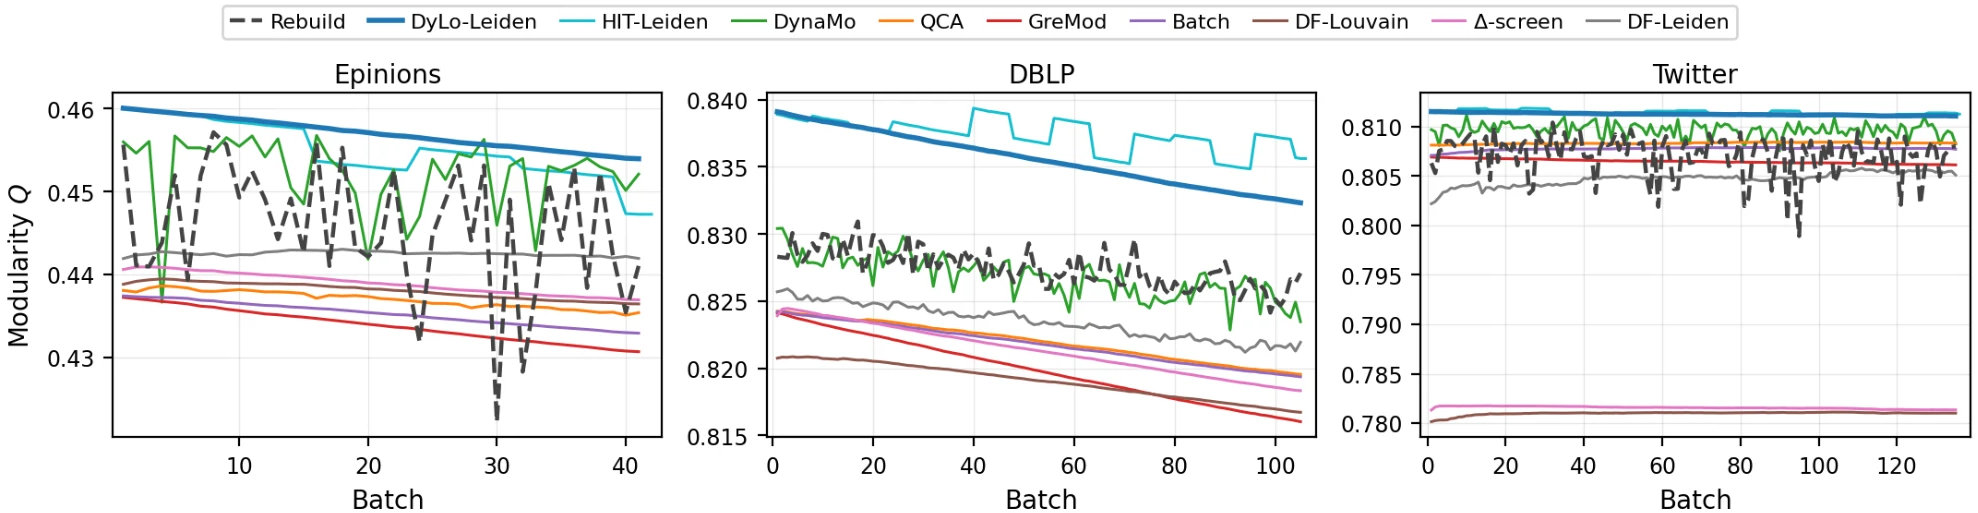
\includegraphics[width=\linewidth]{figures/q_trend.png}
\caption{\textbf{Exp-1.} Per-batch modularity $Q_t$ along the update stream
(Rebuild: Leiden rerun on each batch).}
\Description{Three line charts side by side of modularity against batch index
for Epinions, DBLP, and Twitter, one line per method, with a shared legend on
top. DyLo-Leiden and HIT-Leiden are on top in every panel; the dashed rebuild
line fluctuates strongly; GreMod is near the bottom.}
\label{fig:qtrend}
\end{figure}

% Five-panel row: Exp-4, Exp-2b, and the Exp-3 frontier (fig:knee).
\begin{figure*}[!tb]\centering
% Panels (a-d) from scripts/make_fig_exp4_row.py; (e) from make_fig_exp3_frontier.py.
\begin{subfigure}[t]{0.192\textwidth}\centering
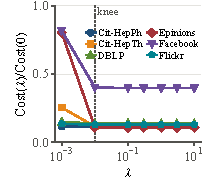
\includegraphics[width=\linewidth]{figures/exp4_cost.pdf}
\caption{Exp-4: cost.}
\end{subfigure}\hfill
\begin{subfigure}[t]{0.192\textwidth}\centering
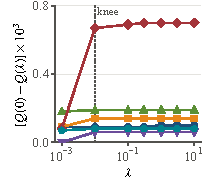
\includegraphics[width=\linewidth]{figures/exp4_qloss.pdf}
\caption{Exp-4: $\bar Q$ loss.}
\end{subfigure}\hfill
\begin{subfigure}[t]{0.192\textwidth}\centering
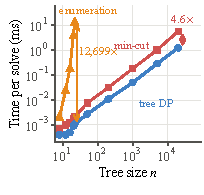
\includegraphics[width=\linewidth]{figures/exp2b_scaling.pdf}
\caption{Exp-2b: scaling.}
\end{subfigure}\hfill
\begin{subfigure}[t]{0.192\textwidth}\centering
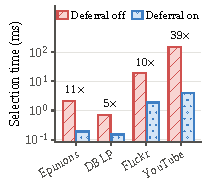
\includegraphics[width=\linewidth]{figures/exp2b_seltime.pdf}
\caption{Exp-2b: streams.}
\end{subfigure}\hfill
\begin{subfigure}[t]{0.192\textwidth}\centering
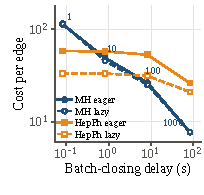
\includegraphics[width=\linewidth]{figures/exp3_frontier.pdf}
\caption{Exp-3: batching.}
\label{fig:exp3}
\end{subfigure}
\caption{(a, b) \textbf{Exp-4.} Exchange-rate sensitivity in structural cost and stream-mean modularity (dotted: knee);
(c, d) \textbf{Exp-2b.} Selector time on synthetic trees ($n\le22$ binned) and
real streams with source deferral off/on;
(e) \textbf{Exp-3.} Structural work per edge versus approximate batch-closing
delay at $\lambda=0$ (labels: batch size; MH: MultiHop-RAG; HepPh: Cit-HepPh).}
\Description{Five panels. Panels a and b plot relative structural cost
and modularity loss against the exchange rate on a log axis for six graphs;
all curves flatten after a knee at 0.01. Panel c plots time per solve against
tree size on log-log axes: enumeration rises steeply and is 12,699 times
slower than tree DP at 22 nodes, while min-cut closure stays 1.7 to 4.6 times
slower than tree DP up to 20,000 nodes. Panel d compares deferral-off and
deferral-on selection time for Epinions, DBLP, Flickr, and YouTube, with
speedups of 11, 5, 10, and 39 times. Panel e plots the eager and lazy
cost-delay frontiers for MultiHop-RAG and Cit-HepPh at batch sizes 1, 10,
100, and 1000; larger batches reduce work per edge while increasing delay.}
\label{fig:knee}
\end{figure*}

\stitle{Quality along the stream.} On Epinions, DBLP, and Twitter,
\DyLo{}-Leiden's per-batch $Q_t$ is at most $0.005$ below HIT-Leiden's
(Figure~\ref{fig:qtrend}). Rebuild reruns the detector after each batch;
its modularity fluctuates more across the stream.

\begin{table}[tb]
\centering
\caption{\textbf{Exp-2.} Component ablation (five-run means).}
\label{tab:ablation}
\begin{scriptsize}
\setlength{\tabcolsep}{0.25em}
\begin{tabular*}{\linewidth}{@{\extracolsep{\fill}}clrrc@{}}
\toprule
Variant & Removed & Latency (ms) & $\Delta\mathsf C$ & Commit \\
\midrule
$V_0$ & ---          & $4.72/9.60/27.4$ & $.133/.046/.057$ & --- \\
\midrule
$V_1$ & certificates & $11.4/17.4/43.5$ & $.133/.046/.057$ & same \\
$V_2$ & cost tree    & $6.07/15.9/57.9$ & $.133/.046/.057$ & same \\
$V_3$ & pruning      & $7.66/13.0/39.3$ & $.144/.050/.061$ & changed \\
\bottomrule
\end{tabular*}
\par\smallskip\raggedright
Triplets: Epinions/Flickr/YouTube. Every arm has rounded
$\bar Q=.4559/.6692/.7277$. $\Delta\mathsf C$: mean normalized accrued
structural cost per batch; ``same'' refers to the committed sets.
\end{scriptsize}
\end{table}

\stitle{Exp-2: Implementation speedups.}
Removing certificates raises latency to $1.59$--$2.42\times$ that of $V_0$;
removing incremental cost-tree maintenance raises it to $1.29$--$2.11\times$
(Table~\ref{tab:ablation}). Each ablation removes one optimization. Both
preserve the recorded partitions and structural scores. Pruning reduces
latency and cost, with different committed sets at the same reported
$\bar Q$: it preserves the frozen objective's optimum but can change the
chosen maximizer and subsequent trajectory.

\stitle{Certified frontier in practice.} Across nine graphs excluding
LiveJournal, \DyLo{}-Leiden's median frontiers contain $1{,}287$--$5{,}450$ vertices per batch
of up to $10^3$ edges (first $40$ batches, or the full shorter stream).
Counts include all vertices entering gain-proposal evaluation, deduplicated
across rounds. On DBLP, Flickr, and YouTube, the medians are below $1\%$ of
vertices. Certificate gating skips $91.8$--$99.9\%$ of endpoint rechecks
(Appendix~\ref{app:frontier}).

% Integrated from the author-supplied experiment, 2026-09-24.
% Author clarified: 5,000 total small-instance comparisons; same environment
% and timing scope as the manuscript. Original preserved under output/.
\stitle{Exp-2b: Exact selection through the single-anchor reduction.}
\label{sec:exp:selector}
\emph{Same-instance exactness and scaling.}
On synthetic forests, we maximize $\sum_{c\in D}(g(c)-\lambda\bar w_t(c))$
over ancestor-closed node sets $D$: selecting a node requires selecting its
ancestors. Gains $g(c)$ are sampled from $U(-10,10)$, $\bar w_t(c)$ is the
fixed marginal refresh weight, and $\lambda\in\{0,0.1,0.5,1,2\}$.
We compare exhaustive enumeration, generic maximum-weight
closure~\cite{picard1976maximal} solved by min-cut, and tree DP on identical
inputs (the objective in Theorem~\ref{thm:dp}).

All three solvers select identical sets in $5{,}000$ tests with $n\le22$;
DP and closure also agree up to $20{,}000$ nodes. DP is fastest at every
measured size (Figure~\ref{fig:knee}(c)): enumeration is $12{,}699\times$
slower at $22$ nodes, and closure is $1.7$--$4.6\times$ slower
(Appendix~\ref{app:defer-seltime}).


\emph{Real-stream selection.}
We compare source deferral off/on over eight full native graph streams
(excluding GPlus and LiveJournal) at $\lambda=0.1$
(three-seed timing medians; on: $\varepsilon=0.05$).
Without deferral, two-anchor actions use min-cut while single-anchor rounds
can use DP; with deferral, all $2{,}079$ reported rounds use DP.
Source deferral reduces total selection time by up to $39\times$ on YouTube
(Figure~\ref{fig:knee}(d)), with potentially different solver inputs.
YouTube's driver latency falls from $27.2$ to $26.9$\,ms per batch.
Driver timing includes graph maintenance and index emission; main-table
latency excludes partition output (Appendix~\ref{app:defer-seltime}).

Across eight graphs and three detector instances, cumulative cost, including
executed refreshes and closing pending liabilities, agrees on $23$ of $24$
deferral pairs and is $0.01\%$ higher for Epinions/\Louvain{}. Every pair
agrees in $\bar Q$ to five decimals.


\stitle{Selector fidelity.} Validation accepts all $1{,}437$ nonempty groups
proposed across eight graphs and three instances, without invoking
\textsc{Peel}. Per-destination greedy selection matches tree DP at the
default rate. At smaller rates, DP gains $32$--$100\%$ in surrogate objective
by sharing ancestor openings.

% Temporarily hidden (2026-09-23): Exp-2c is not required for the
% single-anchor / exact-DP contribution. Preserve the source for restoration.
% \input{tabepssweep}

\stitle{Exp-3: Batch size and batch-closing delay.}
\label{sec:exp:batch}
At $\lambda=0$, we vary $E\in\{1,10,100,1000\}$ on the MultiHop-RAG
news graph and Cit-HepPh (Figure~\ref{fig:knee}(e)). On the news graph,
increasing $E$ from $1$ to $1000$ lowers structural work from $113.5$ to
$7.74$ per edge but raises approximate batch-closing delay from $0.08$ to
$82.8$\,s. Larger batches amortize refresh work but postpone index freshness;
lazy evaluation further favors small batches when updates are localized,
as on Cit-HepPh. Delays end at batch closure, before maintenance and
summary generation; the arrival-rate model and default-rate results are
in Appendix~\ref{app:exp3-detail}.

\stitle{Exp-4: Sensitivity to the exchange rate.}
Figure~\ref{fig:knee}(a, b) sweeps $\lambda$ on Cit-HepPh, Cit-HepTh, DBLP,
Epinions, Facebook, and Flickr, reporting
$\mathrm{Cost}(\lambda)/\mathrm{Cost}(0)$ and $\bar Q(0)-\bar Q(\lambda)$.
At $\lambda=10^{-2}$, five graphs save $86$--$89\%$ of structural work with
mean-modularity losses of $0.06$--$0.67\times10^{-3}$; Facebook's cost ratio
is $0.402$. The curves flatten beyond this knee, motivating the shared
default $\lambda=10^{-1}$ (Appendix~\ref{app:exp4-detail}). Each reference
is the same sweep's $\lambda=0$ run.

\subsection{Case study: Maintenance efficiency and sensemaking quality}
\label{sec:exp:e2e}

\begin{comment}

\stitle{Exp-6 \& Exp-7: Token cost and answer quality on HotpotQA.} We evaluate a HotpotQA~\cite{yang2018hotpotqa} GraphRAG index under a $20$-batch stream (Table~\ref{tab:tokens}), measuring the input tokens of every regenerated summary.

\emph{Token cost.} \DyLo{}-Leiden regenerates $51.8$k input tokens per batch, $83.7\%$ fewer than from-scratch. DF-\Louvain{} and $\Delta$-screen appear inexpensive partly because more than $82\%$ of their communities remain unchanged; \DyLo{} retains only $29.5\%$ unchanged yet still regenerates the fewest tokens by selecting cheaper communities.

\begin{table}[tb]\centering
\caption{\textbf{Exp-7.} LLM input tokens per batch on the HotpotQA index
(GPT-4o-mini input rate: \$0.15/M~\cite{openai2024gpt4omini}); the lower block reports answer quality on the same index.}
\label{tab:tokens}
\begin{footnotesize}
\setlength{\tabcolsep}{0.35em}
\resizebox{\linewidth}{!}{%
\begin{tabular}{lrrrrr}
\toprule
Method & Unch.\ (\%) & Comms/b. & Tokens/b. & \$/b. & Saved (\%) \\
\midrule
From-scratch Leiden & --- & $826$ & $317{,}662$ & $0.0476$ & --- \\
\midrule
\DynaMo{}       & $71.9$ & $118$ & $147{,}798$ & $0.0222$ & $53.5$ \\
DF-Leiden       & $72.9$ & $98$  & $125{,}388$ & $0.0188$ & $60.5$ \\
HIT-Leiden      & $20.6$ & $225$ & $111{,}063$ & $0.0167$ & $65.0$ \\
\GreMod{}       & $53.6$ & $127$ & $90{,}379$  & $0.0136$ & $71.5$ \\
\QCA{}          & $39.7$ & $96$  & $82{,}146$  & $0.0123$ & $74.1$ \\
\Batch{}        & $75.0$ & $64$  & $74{,}563$  & $0.0112$ & $76.5$ \\
$\Delta$-screen & $82.5$ & $54$  & $72{,}698$  & $0.0109$ & $77.1$ \\
DF-\Louvain{}   & $\mathbf{82.6}$ & $45$ & $59{,}696$ & $0.0090$ & $81.2$ \\
\midrule
\DyLo{}-Leiden  & $29.5$ & $322$ & $\mathbf{51{,}827}$ & $\mathbf{0.0078}$ & $\mathbf{83.7}$ \\
\midrule
\multicolumn{6}{l}{\emph{Answer quality on the same index ($306$ questions)}} \\
\cmidrule(lr){1-6}
Index & Unch.\ (\%) & $F_1$ & EM & UNKNOWN & W/L/T \\
\midrule
All-fresh         & ---    & $.0769$ & $.0490$ & $79.7\%$ & --- \\
\DyLo{}           & $29.5$ & $\mathbf{.0817}$ & $\mathbf{.0523}$ & $\mathbf{78.4\%}$ & $5/4/297$ \\
Mask-$40$ control & ---    & $.0444$ & $.0327$ & $87.9\%$ & $22/9/275$ \\
\bottomrule
\end{tabular}}
\end{footnotesize}
\end{table}

\emph{Answer quality.} Against the same partition with every summary refreshed, \DyLo{}'s selective index is statistically indistinguishable over $306$ questions (paired token-$F_1$ $\Delta=-.0047$, $95\%$ CI $[-.016,+.007]$; $5/4/297$, $p=1.000$). In contrast, blanking $40\%$ of summaries reduces token-$F_1$ by $.0326$ ($p=.029$), showing that the evaluation detects semantic loss but no penalty from \DyLo{}'s selective deferral.
\FloatBarrier

\end{comment}

\stitle{Exp-5: Measured maintenance and sensemaking quality.}
We update a GraphRAG index from $304$ to $327$ articles drawn from the
MultiHop-RAG news corpus~\cite{tang2024multihoprag}. All eight arms use
the same extracted graph and Qwen2.5-32B-Instruct~\cite{yang2024qwen25}
for both initial and updated community reports.
Under the archived eager-source policy, incremental arms reuse reports with
unchanged community membership; Rebuild regenerates all reports. Each arm
runs alone on an H100 with four concurrent requests and both response and
prefix caching disabled (Appendix~\ref{app:exp5-detail}).

\begin{table}[tb]\centering
\caption{\textbf{Exp-5.} Measured GraphRAG maintenance.}
\label{tab:arena-main}
\footnotesize
\setlength{\tabcolsep}{0.25em}
\begin{tabular*}{\linewidth}{@{\extracolsep{\fill}}lrrrrr@{}}
\toprule
Method & Calls & $T_s$ (s) & $T_s/T_m$ (\%) & Tok. (k) & $T_m$ (s) \\
\midrule
Rebuild & 1637 & 7495.8 & 99.63 & 2,630.2 & 7523.5 \\
HIT-Leiden & 721 & 3467.6 & 99.27 & 1,448.9 & 3493.1 \\
\DynaMo{} & 717 & 3473.0 & 99.27 & 1,464.2 & 3498.7 \\
\QCA{} & 695 & 3360.4 & 99.23 & 1,411.8 & 3386.3 \\
DF-\Louvain{} & 717 & 3476.0 & 99.26 & 1,478.0 & 3501.8 \\
$\Delta$-screen & 732 & 3565.0 & 99.29 & 1,501.1 & 3590.6 \\
\Batch{} & 712 & 3438.9 & 99.25 & 1,442.2 & 3464.8 \\
\DyLo{} & $\mathbf{344}$ & $\mathbf{1901.1}$ & 98.68 & $\mathbf{1,083.3}$ & $\mathbf{1926.5}$ \\
\bottomrule
\end{tabular*}
\par\smallskip\raggedright
$T_s$: re-summarization time; $T_m$: graph-ready to queryable maintenance.
Calls and tokens count successful update summaries (native input plus output).
Initial construction, extraction, and old-report repair are excluded; retry
time is included. One run per arm.
\end{table}

\emph{Maintenance savings.} Re-summarization takes $98.68$--$99.63\%$ of
maintenance time (Table~\ref{tab:arena-main}). Relative to \QCA{}, the
strongest incremental baseline, and Rebuild, \DyLo{} reduces
re-summarization time by $43.4\%$ and $74.6\%$, and successful update-summary
tokens by $23.3\%$ and $58.8\%$, respectively. Because re-summarization
dominates wall time, these savings carry through to complete graph-ready
maintenance.

\emph{Sensemaking quality.} We evaluate the first $60$ archived synthesis
questions ($q_0$--$q_{59}$)
with GraphRAG global search~\cite{edge2024graphrag}, using each index's
complete root-report cut and the 32B answer generator, with $8{,}000$-token
budgets per map chunk and for reduce evidence. \DyLo{} uses eight map
chunks per question; each baseline uses four
(Appendix~\ref{app:exp5-detail}). An independent local \texttt{gpt-oss-120b} judge
compares anonymized answers in both orders on comprehensiveness (coverage),
diversity (perspectives), empowerment (support for informed judgment), and
directness (focus on the question).

\begin{table}[tb]\centering
\caption{\textbf{Exp-5.} DyLo preference against each baseline ($\uparrow$).}
\label{tab:sensemaking-current}
\footnotesize
\setlength{\tabcolsep}{0.25em}
% Equal superscript space keeps marked and unmarked scores aligned.
\begin{tabular*}{\linewidth}{@{\extracolsep{\fill}}lrrrr@{}}
\toprule
Opponent & Comp. & Div. & Emp. & Dir. \\
\midrule
\Batch{} & $64.17^{+}$ & $59.17^{\phantom{+}}$ & $60.83^{+}$ & $61.25^{+}$ \\
Rebuild & $65.42^{+}$ & $57.08^{\phantom{+}}$ & $63.33^{+}$ & $63.75^{+}$ \\
HIT-Leiden & $58.33^{\phantom{+}}$ & $49.58^{\phantom{+}}$ & $58.75^{\phantom{+}}$ & $57.92^{\phantom{+}}$ \\
\DynaMo{} & $65.42^{+}$ & $56.25^{\phantom{+}}$ & $67.92^{+}$ & $56.25^{\phantom{+}}$ \\
\QCA{} & $65.42^{+}$ & $64.17^{+}$ & $60.42^{+}$ & $58.75^{\phantom{+}}$ \\
DF-\Louvain{} & $67.50^{+}$ & $60.42^{\phantom{+}}$ & $64.58^{+}$ & $66.67^{+}$ \\
$\Delta$-screen & $66.25^{+}$ & $60.42^{\phantom{+}}$ & $64.58^{+}$ & $61.25^{+}$ \\
\bottomrule
\end{tabular*}
\par\smallskip\raggedright
Win/tie/loss scores are $100/50/0$, averaged over both orders within each
question, then over $60$ questions; $50$ denotes equal preference. Unadjusted
$95\%$ intervals use $10{,}000$ question-bootstrap resamples with both orders
kept together; $^{+}/^{-}$ marks intervals wholly above/below $50$
(Appendix~\ref{app:exp5-detail}).
\end{table}

The unadjusted $95\%$ intervals favor \DyLo{} in comprehensiveness and
empowerment against \Batch{}, Rebuild, and \QCA{}, in directness against
\Batch{} and Rebuild, and in diversity against \QCA{}. The remaining
intervals for these three baselines and all four against HIT-Leiden
include or touch $50$. These local-judge results support competitive
sensemaking quality at lower maintenance cost.


% Allow the next section to follow without flushing an incomplete column.
